\documentclass[12pt]{article}
\usepackage[english]{babel}
\usepackage[utf8x]{inputenc}
\usepackage{amsmath}
\usepackage{graphicx}     % Used to for importing images
\usepackage{indentfirst}  % Indents 1st paragraph (by default its off)
\usepackage{longtable}    % Tables than can span over multiple pages

% Define Global Variables
\setlength{\parindent}{20pt}
\graphicspath{ {/Diagrams} }

\begin{document}

\begin{titlepage}

% Defines a new command to draw horizontal lines
\newcommand{\Line}{\rule{\linewidth}{0.5mm}} 

% Center everything on the page
\center
 
% textsc - capitalizes every letter
\textsc{\LARGE University of Gothenburg}
% Define gap after text line
\\[3.5cm] 

% Course code and name
\textsc{\Large DIT168}\\[0.3cm]
\textsc{\large Project: Industrial IT and Embedded Systems}\\[0.5cm]

% Use the defined command to draw lines
\Line \\[0.4cm]
{\huge \bfseries Software Architectural Document}\\[0.4cm]
\Line \\[0.5cm]
 
% Large italic text
\Large \textit{Authors:}
\\Erik Laurin
\\Isabelle Törnqvist
\\Joacim Eberlen
\\Justinas Stirbys \\[4cm]

% Original date for the vision
{\large Group 01} \\[0.3cm]
{\large March 30th, 2018}

% Fills the remaining page with whitespace
\vfill

\end{titlepage}

% Creating table of contents
\tableofcontents
\pagebreak

% SAD start
%%%%%%%%%%%%%%%%%%%%%%%%%%%%%%%%%%
% Add SAD history of changes table
%%%%%%%%%%%%%%%%%%%%%%%%%%%%%%%%%%

\section{Revision History}
The evolution of the Software Architectural Document for project dashFTABs is detailed under this section. Emphasis is put on changes incorporated, via Description column, the date and the author. In situation where all members have contributed to a change the author will be listed as Group 01.
% Define 4 aligned columns; l = left, c = center, r = right, the | = means vertical line    % \hline -> Draw horizontal line
% p{xcm} -> specifies how much space the column should take up, 
% 0.x\linewidth is used to make it p{} command more dynamic
\begin{longtable}{ | p{0.25\linewidth} | p{0.1\linewidth} | p{0.5\linewidth} | p{0.15\linewidth} | }\hline 
    Date & Version & Description & Author \\ \hline
    27th March, 2018 & 0.1 & Added Functional Requirements & Group 01\\ \hline
    4th April, 2018 & 0.2 & Added Introduction & Justinas\\ \hline
    5th April, 2018 & 0.3 & Added Use Case View & Justinas\\ \hline
    12th April, 2018 & 0.4 & Added Sequence Diagrams0 for UC1-UC3 & Justinas\\ \hline
\end{longtable}
\pagebreak

%%%%%%%%%%%%%%%%%%%%%%%%%%%%%%
% Adding document introduction
%%%%%%%%%%%%%%%%%%%%%%%%%%%%%%
\section{Introduction}
\subsection{Purpose}
The purpose of this document is to familiarize the reader with the architectural overview of the software, developed for the project dashFTABs, by examining different architectural viewpoints. In continuation, the document includes architectural drivers, such as system requirements, and attempts to identify significant dashFTABs system’s behaviour.\par

\subsection{Scope}
  The software was developed as part of the DIT168 Project: Industrial IT and Embedded Systems course taught at University of Gothenburg in Gothenburg, Sweden. The project course provides a 3D printed miniature car, dubbed Dash by the project group. The project groups communicate amongst each other to implement a Vehicle-to-Vehicle (V2V) protocol. Moreover, via incorporation of the protocol the project groups must expand Dash’s functional capabilities by implement platooning.\par

\subsection{Audience}
  The document contains technical details of the project and utilizes Unified Modeling Language (UML for short) to express architecture. Therefore, the reader must possess some minimal or introductory knowledge of UML. As such the intended readers are members or somewhat affiliated with software engineering. Moreover, the document is intended for the project’s stakeholders, which include, but not exclusively, the development team, the course representatives and the teaching assistants.
\pagebreak

%%%%%%%%%%%%%%%%%%%%%%%%%%%%%%%%%%%%%%%%%%%%%%%%%%%
% Adding section detailing architecture motivations
%%%%%%%%%%%%%%%%%%%%%%%%%%%%%%%%%%%%%%%%%%%%%%%%%%%
\section{Architectural Drivers}
\subsection{Functional Requirements}
Functional requirements were used to identify and narrow down the project scope. The requirements are prioritized using MoSCoW notation i.e. requirements are divided into Must, Shoulds, Coulds, and Wont’s. Must dictates requirements that are mandatory for the final demonstration. Should expresses requirements that are significant, but do not have a defined deadline. Could expresses requirements/features that would improve the project quality, but are not necessarily implemented. Lastly, Won’t is used to track identified requirements that will not be implemented, due to product owner dislike or disapproval, time and budgetary constraints.\par

% Functional requirement table
% Define 4 aligned columns; l = left, c = center, r = right, the | = means vertical line    % \hline -> Draw horizontal line
\begin{longtable}{| p{0.05\linewidth} | p{0.15\linewidth} | p{0.45\linewidth} | p{0.25\linewidth} | p{0.1\linewidth} |}\hline 
    ID & Requirement & Description & Status & Priority \\ \hline
    F1 & Message Log & A web page must contain a message log of everything that has been sent internally and externally within the car & Not Implemented & Must\\ \hline
    F2 & Remote Controller & A web page must contain a graphical remote controller that communicates and controls Dash, when the car is the leader of the platoon & Not Implemented & Must\\ \hline
    F3 & Ultrasonics & Dash will support ultrasonic sensors; will be able to broadcast distance sensor data to the local OD4 session & Not Implemented & Must\\ \hline
    F4 & Leader Connection & The car, Dash, must be able to support Leader functionality (i.e. send LeaderStatus requests) while platooning & Not Implemented & Must\\ \hline       
    F5 & Follower Connection & The car, Dash, must be able to participate in platooning as a follower & Not Implemented & Must\\ \hline
    F6 & Maneuvering & The car will drive forward, turn left or right on commands received over the OD4 session & Not Implemented & Must\\ \hline
    F7 & IMU & Dash must be able to use the IMU on its BeagleBoard Blue to calculate the distance moved and be able to send that using the V2V Protocol & Not Implemented & Must\\ \hline
    F8 & V2V Protocol & The car must be able to support the V2V Protocol. It is required for it to communicate with other cars and send sensors data & Not Implemented & Must\\ \hline
    F9 & Collision Prevention & Dash will stop/brake when ultrasonic readings return an object that is less or equals to 10 cm ahead & Not Implemented & Should\\ \hline
    F10 & Emergency Brake & The car will stop if it fails to receive 3 update requests (i.e. hasn’t received anything in 300ms) and/or the connection to other cars has been lost & Not Implemented & Must\\ \hline
    F11 & Video Streaming& The car could incorporate the RPi and camera to live stream it’s video & Not Implemented & Could\\ \hline
    F12 & Lane Following & Via incorporation of the RPi camera, Dash could implement identification and following of straight lines & Not Implemented & Could\\ \hline
\end{longtable}

%%%%%%%%%%%%%%%%%%%%%%%%%%%%%%%%%%%%%%%%
% Adding section about project use cases
%%%%%%%%%%%%%%%%%%%%%%%%%%%%%%%%%%%%%%%%
\section{Use Case View}
This document section attempts to identify the main behaviour exhibited by Dash. This is done by expressing the behaviour as use case scenarios. The chosen scenarios depicts some of the significant features of developed project. Moreover, the identified scenarios all utilize the V2V Protocol in different aspects, meaning the use case scenarios use different messages from the protocol. Therefore, the identified scenarios fulfil different aspects of the functional requirements of F8 (V2V Protocol).\par

\subsection{Use Case Scenarios}

%%% Use Case 1 Table
\subsubsection{Connect As Follower}
\begin{longtable}{| p{0.2\linewidth} | p{0.8\linewidth} |}\hline 
    ID & UC1\\ \hline
    Use Case & Connect as Follower\\ \hline
    Description & Dash connects to another miniature car as a Follower and begins to receiving Leader Status update messages\\ \hline
    Actors & Dash, Another Car\\ \hline
    Preconditions & Excluding Dash there is another miniature car with the V2V protocol that are not already connected to any cars\\ \hline
    Steps & Basic Flow: \begin{enumerate} % enumerate creates a numbered list
      \itemsep 0em % -> Specify gaps between numbers in list 
      \item Dash uses Announce Presence (it’s not very effective). Another car receives Dash’s IP and group number
    \item Another Car announces presence. Dash receives it’s IP and group number
        \item Dash uses Follow Requests. Selects which group car to follow
        \item Another Car receives follow request and does not have a follower yet. Another Car sends Follow Response
        \item A connection using UDP Sender and Receiver is established between Dash and Another Car 
        \end{enumerate}
        Alternative Flow: \begin{enumerate}
          \setcounter{enumi}{3} % -> Starts list from a different specified index + 1
          \item Another Car already has a Follower. 
            \begin{enumerate} % -> nested enumerates, index list. Default index 1->a->i->A
              \itemsep 0em % -> Specify gaps between numbers in list 
            \item No Follower Request is sent
            \item Display a message informing the users
                \item Continues at Basic Flow 2
          \end{enumerate}
        \end{enumerate}\\ \hline
\end{longtable}

%%% Use Case 2 Table
\subsubsection{Connect As Leader}
\begin{longtable}{| p{0.2\linewidth} | p{0.8\linewidth} |}\hline 
    ID & UC2\\ \hline
    Use Case & Connect as Leader\\ \hline
    Description & Dash connects to another miniature car as a Leader and begins to sending Leader Status update messages\\ \hline
    Actors & Dash, Another Car\\ \hline
    Preconditions & Excluding Dash there is another miniature car with the V2V protocol that are not already connected to any cars\\ \hline
    Steps & Basic Flow: \begin{enumerate} % enumerate creates a numbered list
        \itemsep 0em % -> Specify gaps between numbers in list 
      \item Dash uses Announce Presence (it’s not very effective). Another car receives Dash’s IP and group number
    \item Another Car announces presence. Dash receives it’s IP and group number
        \item Dash receives follow request and does not have a follower yet. Dash sends Follow Response
        \item Another Car receives follow request and does not have a follower yet. Another Car sends Follow Response
        \item A connection using UDP Sender and Receiver is established between Dash and Another Car 
        \end{enumerate}
        Alternative Flow: \begin{enumerate}
          \setcounter{enumi}{3} % -> Starts list from a different specified index + 1
          \item Dash already has a Follower. 
            \begin{enumerate} % -> nested enumerates, index list. Default index 1->a->i->A
              \itemsep 0em % -> Specify gaps between numbers in list 
            \item No Follower Request is sent
            \item Display a message informing the users
                \item Continues at Basic Flow 2
          \end{enumerate}
        \end{enumerate}\\ \hline
\end{longtable}

%%% Use Case 3 Table
\subsubsection{Stop Following Leader}
\begin{longtable}{| p{0.2\linewidth} | p{0.8\linewidth} |}\hline 
    ID & UC3\\ \hline
    Use Case & Connect as Leader\\ \hline
    Description & Dash disconnect from Another Car, which acted as a Leader\\ \hline
    Actors & Dash, Another Car\\ \hline
    Preconditions & Dash is already connected as a Follower to Another Car\\ \hline
    Steps & Basic Flow: \begin{enumerate} % enumerate creates a numbered list
        \itemsep 0em % -> Specify gaps between numbers in list 
      \item Dash sends Follower Status and receives Leader Status, indicating it’s following Another Car
    \item Dash sends Stop Following message and stops moving
        \item Dash removes Another Car as it’s leader
        \item Another Car receives stop following message. Another Car removes Dash as it’s follower
  \end{enumerate}\\ \hline
\end{longtable}

%%% Use Case 4 Table
\subsubsection{Stop Following Leader}
\begin{longtable}{| p{0.2\linewidth} | p{0.8\linewidth} |}\hline 
    ID & UC4\\ \hline
    Use Case & Drive Dash\\ \hline
    Description & Another Car connects to Dash as a Follower, at which point a Driver uses the remote controller to maneuver Dash\\ \hline
    Actors & Dash, Driver, Another Car\\ \hline
    Preconditions & Another Car is already connected to Dash as a Follower\\ \hline
    Steps & Basic Flow: \begin{enumerate} % enumerate creates a numbered list
        \itemsep 0em % -> Specify gaps between numbers in list 
      \item ???
  \end{enumerate}\\ \hline
\end{longtable}

\subsection{Use Case Diagram}
To depict use case interactions amongst each other, a use case diagram was created. Moreover, the diagram also servers as a visual aid, aimed to improve understanding of actor interactions with project functionality. The diagram depicts the interactions between the most significant use cases, mentioned in previous sections.\par

% Adding use case diagram image
\begin{figure}
\centering
% Make image as wide as the line
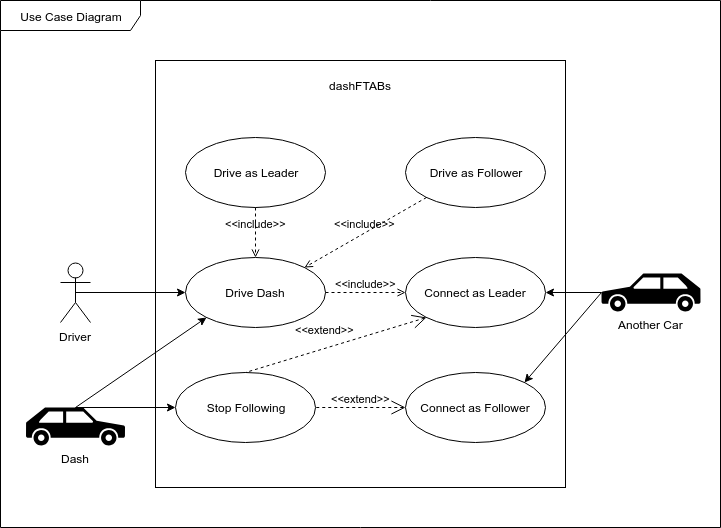
\includegraphics[width=\linewidth]{Diagrams/UseCaseDiagram.png}
\caption{Use Case Diagram}
\label{fig:usecasediagram}
\end{figure}


\end{document}